\makeatletter
\@ifundefined{standalonetrue}{\newif\ifstandalone}{}
\@ifundefined{section}{\standalonetrue}{\standalonefalse}
\makeatother
\ifstandalone
\documentclass{report}

\usepackage{textcase}
\usepackage[pdftex]{graphicx}
%\usepackage{hyperref}
%\hypersetup{breaklinks=true}


% Added packages
\usepackage[usenames]{color}
\usepackage{amsfonts, amsmath, amssymb, graphics}

% NOTE: bibentry MUST appear before the hyperref or build will fail
\usepackage{bibentry}
\nobibliography*
\usepackage[square,sort,comma,numbers]{natbib}
  
\usepackage{float}
\usepackage[
    hyperindex=true,		% Make numbers of index links as well
   	backref=page, 		% Provide page listing where refs occur in the bibliography
	%breaklinks=true,
    colorlinks,%
    citecolor=green,%
    filecolor=blue,%
    linkcolor=red,%
    urlcolor=red, 
]{hyperref}

\usepackage{dsfont}
%%%% USEPACKAGES for MACROS %%%%%
\usepackage{algpseudocode}
\usepackage[chapter]{algorithm}
\usepackage{caption}
\usepackage{subcaption}
\usepackage{url}

\usepackage{array}
\usepackage{arydshln}
\usepackage{multirow}
\usepackage{multicol}
\usepackage[section]{placeins}

\newcommand{\toprule}[0]{\hline}
\newcommand{\midrule}[0]{\hline\hline}
\newcommand{\bottomrule}[0]{\hline}

\DeclareSymbolFont{AMSb}{U}{msb}{m}{n}
\DeclareMathSymbol{\N}{\mathbin}{AMSb}{"4E}
\DeclareMathSymbol{\Z}{\mathbin}{AMSb}{"5A}
\DeclareMathSymbol{\R}{\mathbin}{AMSb}{"52}
\DeclareMathSymbol{\Q}{\mathbin}{AMSb}{"51}
\DeclareMathSymbol{\PP}{\mathbin}{AMSb}{"50}
\DeclareMathSymbol{\I}{\mathbin}{AMSb}{"49}
%\DeclareMathSymbol{\C}{\mathbin}{AMSb}{"43}

%%%%%% VECTOR NORM: %%%%%%%
\newcommand{\vectornorm}[1]{\left|\left|#1\right|\right|}
\newcommand{\vnorm}[1]{\left|\left|#1\right|\right|}
\newcommand{\by}[0]{\times}
\newcommand{\vect}[1]{\mathbf{#1}}
%\newcommand{\mat}[1]{\mathbf{#1}} 

%\renewcommand{\vec}[1]{ \textbf{#1} }
%%%%%%%%%%%%%%%%%%%%%%

%%%%%%% THM, COR, DEF %%%%%%%
%\newtheorem{theorem}{Theorem}[section]
%\newtheorem{lemma}[theorem]{Lemma}
%\newtheorem{proposition}[theorem]{Proposition}
%\newtheorem{corollary}[theorem]{Corollary}
%\newenvironment{proof}[1][Proof]{\begin{trivlist}
%\item[\hskip \labelsep {\bfseries #1}]}{\end{trivlist}}
%\newenvironment{definition}[1][Definition]{\begin{trivlist}
%\item[\hskip \labelsep {\bfseries #1}]}{\end{trivlist}}
%\newenvironment{example}[1][Example]{\begin{trivlist}
%\item[\hskip \labelsep {\bfseries #1}]}{\end{trivlist}}
%\newenvironment{remark}[1][Remark]{\begin{trivlist}
%\item[\hskip \labelsep {\bfseries #1}]}{\end{trivlist}}
%\newcommand{\qed}{\nobreak \ifvmode \relax \else
%      \ifdim\lastskip<1.5em \hskip-\lastskip
%      \hskip1.5em plus0em minus0.5em \fi \nobreak
%      \vrule height0.75em width0.5em depth0.25em\fi}
%%%%%%%%%%%%%%%%%%%%%%


% \DeclareMathOperator{\Sample}{Sample}
%\let\vaccent=\v % rename builtin command \v{} to \vaccent{}
%\renewcommand{\vec}[1]{\ensuremath{\mathbf{#1}}} % for vectors
\newcommand{\gv}[1]{\ensuremath{\mbox{\boldmath$ #1 $}}} 
% for vectors of Greek letters
\newcommand{\uv}[1]{\ensuremath{\mathbf{\hat{#1}}}} % for unit vector
\newcommand{\abs}[1]{\left| #1 \right|} % for absolute value
\newcommand{\avg}[1]{\left< #1 \right>} % for average
\let\underdot=\d % rename builtin command \d{} to \underdot{}
\renewcommand{\d}[2]{\frac{d #1}{d #2}} % for derivatives
\newcommand{\dd}[2]{\frac{d^2 #1}{d #2^2}} % for double derivatives
\newcommand{\pd}[2]{\frac{\partial #1}{\partial #2}} 
% for partial derivatives
\newcommand{\pdd}[2]{\frac{\partial^2 #1}{\partial #2^2}} 
\newcommand{\pdda}[3]{\frac{\partial^2 #1}{\partial #2 \partial #3}} 
% for double partial derivatives
\newcommand{\pdc}[3]{\left( \frac{\partial #1}{\partial #2}
 \right)_{#3}} % for thermodynamic partial derivatives
\newcommand{\ket}[1]{\left| #1 \right>} % for Dirac bras
\newcommand{\bra}[1]{\left< #1 \right|} % for Dirac kets
\newcommand{\braket}[2]{\left< #1 \vphantom{#2} \right|
 \left. #2 \vphantom{#1} \right>} % for Dirac brackets
\newcommand{\matrixel}[3]{\left< #1 \vphantom{#2#3} \right|
 #2 \left| #3 \vphantom{#1#2} \right>} % for Dirac matrix elements
\newcommand{\grad}[1]{\gv{\nabla} #1} % for gradient
\let\divsymb=\div % rename builtin command \div to \divsymb
\renewcommand{\div}[1]{\gv{\nabla} \cdot #1} % for divergence
\newcommand{\curl}[1]{\gv{\nabla} \times #1} % for curl
\let\baraccent=\= % rename builtin command \= to \baraccent
\renewcommand{\=}[1]{\stackrel{#1}{=}} % for putting numbers above =
\newcommand{\diffop}[1]{\mathcal{L}#1}
\newcommand{\boundop}[1]{\mathcal{B}#1}
\newcommand{\rvec}[0]{{\bf r}}

\newcommand{\Interior}[0]{\Omega}
\newcommand{\domain}[0]{\Omega}
\newcommand{\Boundary}[0]{\partial \Omega}
%\newcommand{\Boundary}[0]{\Gamma}

\newcommand{\on}[1]{\hskip1.5em \textrm{ on } #1}

\newcommand{\gemm}{\texttt{GEMM}}
\newcommand{\trmm}{\texttt{TRMM}}
\newcommand{\gesvd}{\texttt{GESVD}}
\newcommand{\geqrf}{\texttt{GEQRF}}


\newcommand{\minitab}[2][l]{\begin{tabular}{#1}#2\end{tabular}}
\newcommand{\comm}[1]{\textcolor{red}{\textit{#1}}}

\newcommand{\nfrac}[2]{
\nicefrac{#1}{#2}
%\frac{#1}{#2}
}

\usepackage{xparse}


%%%%%%%%%%%%%%%
% Show a Author's Note
% USAGE: 
% \incomplete[Optional footnote message to further clarify note]{The text which is currently not finished}
\DeclareDocumentCommand \incomplete{ o m }
{%
\IfNoValueTF {#1}
{\textcolor{red}{Incomplete: \ul{#2}}} 
{\textcolor{red}{Incomplete: \ul{#2}}\footnote{Comment: #1}}%
}
%%%%%%%%%%%%%%%



%%%%%%%%%%%%%%%
% Show a Author's Note
% USAGE: 
% \authnote[Optional footnote message to further clarify note]{The note to your readers}
\DeclareDocumentCommand \authnote { o m }
{%
\IfNoValueTF {#1}
{\textcolor{blue}{Author's Note: \ul{#2}}} 
{\textcolor{blue}{Author's Note: \ul{#2}}\footnote{Comment: #1}}%
}
%%%%%%%%%%%%%%%



%%%%%%%%%%%%%%%
% Strike out text that doesn't belong in the paper
% USAGE: 
% \strike[Optional footnote to state why it doesn't belong]{Text to strike out}
\DeclareDocumentCommand \strike { o m }
{%
\setstcolor{red}
\IfNoValueTF {#1}
{\textcolor{Gray}{\st{#2}}} 
{\textcolor{Gray}{\st{#2}}\footnote{Comment: #1}}%
}
%%%%%%%%%%%%%%%



%
% colors to show the corrections
\newcommand{\red}[1]{\textbf{\textcolor{red}{#1}}}
\newcommand{\blue}[1]{\textbf{\textcolor{blue}{#1}}}
\newcommand{\cyan}[1]{\textbf{\textcolor{cyan}{#1}}}
\newcommand{\green}[1]{\textbf{\textcolor{green}{#1}}}
\newcommand{\magenta}[1]{\textbf{\textcolor{magenta}{#1}}}
\newcommand{\orange}[1]{\textbf{\textcolor{orange}{#1}}}
%%%%%%%%%% DK DK
% comments between authors
\newcommand{\toall}[1]{\textbf{\green{@@@ All: #1 @@@}}}
\newcommand{\toevan}[1]{\textbf{\red{*** Evan: #1 ***}}}
%\newcommand{\toevan}[1]{}  % USE FOR FINAL VERSION
\newcommand{\toe}[1]{\textbf{\red{*** Evan: #1 ***}}}
\newcommand{\tog}[1]{\textbf{\blue{*** Gordon: #1 ***}}}
%\newcommand{\togordon}[1]{\textbf{\blue{*** Gordon: #1 ***}}}
\renewcommand{\ge}[3]{{\textcolor{blue}{*** \textbf{Gordon:}\strike{#1} #2 ***}}\red{(#3)}}
\renewcommand{\ge}[3]{{\textcolor{blue}{#2}}}
\renewcommand{\ge}[3]{{\textcolor{red}{#2}}}
\newcommand{\eb}[3]{{\textcolor{red}{*** \textbf{Evan:}\strike{#1} #2 ***}}\red{(#3)}}
\renewcommand{\eb}[3]{{{\textcolor{red}{#2}}}}
%\def\ge#1#2#3{}{\textbf{\blue{*** Gordon: #2 ***}}}{(#3)}
\newcommand{\gee}[1]{{\bf{\blue{{\em #1}}}}}
\newcommand{\old}[1]{}
\newcommand{\del}[1]{***#1*** }



\input{macros/misc_mac.tex}
\newcommand{\mathsym}[1]{{}}
\newcommand{\unicode}[1]{{}}
\newcommand{\ep}{\epsilon}
\newcommand{\vx}{\mathbf{x}}


\usepackage{tabularx} 
\newcolumntype{C}{>{\centering\arraybackslash}b{1in}}
\newcolumntype{L}{>{\flushleft\arraybackslash}b{1.5in}}
\newcolumntype{R}{>{\flushright\arraybackslash}b{1.5in}}
\newcolumntype{D}{>{\flushright\arraybackslash}b{2.0in}}
\newcolumntype{E}{>{\flushright\arraybackslash}b{1.0in}}


 


\usepackage{xcolor}
% Sepia
\definecolor{myBGcolor}{HTML}{F6F0D6}
\definecolor{myTextcolor}{HTML}{4F452C}
% Dark
%\definecolor{myBGcolor}{HTML}{3E3535}
%\definecolor{myTextcolor}{HTML}{CFECEC}
%\color{myTextcolor}
\pagecolor{myBGcolor}
 

\begin{document}
\fi


\chapter{Neighbor Queries and Node Ordering}


\section{Neighbor Queries} 

As part of the preprocessing stage for RBF-FD, the scattered point cloud must
be analyzed to generate stencils. To generate a stencil, any collection of
nodes can be selected. However, by choosing nodes close to the stencil center
and well balanced around it, we stand to get the best possible approximations
to derivatives. 

Why? well, the approximations are based on differences. Similar to classic FD,
draw a secant connecting two nodes of a stencil. The slope of the secant
determines the gradient at either point or a point in between. In the limit as
the points are moved closer to the same spot, the approximation to the
derivative at that point becomes exact. 

So ideally every RBF-FD stencil will operate on nearest neighbors. One way to
generate nearest neighbors is brute force $O(N^{2})$; very inefficient. 

Alternatives exist including k-D Tree

\subsection{k-D Tree}
Build complexity, seek times. Internal ordering 

We use implementation provided by Andrea Tagliasacchi \cite{tagliasacchi} as a MEX compiled set of routines for Matlab. These same routines are then linked into C/C++. 

\subsection{Locality Sensitive Hashing}

\cite{Connor2009} provide a fast parallel 

\cite{Henke2012} is working on parallel generation. \cite{IanJohnsonThesis} has OpenCL neighbor queries

We started with a CPU implementation to test appropriateness. 

\authnote{Compare performance of stencil generation in C++}

\begin{figure}
\centering
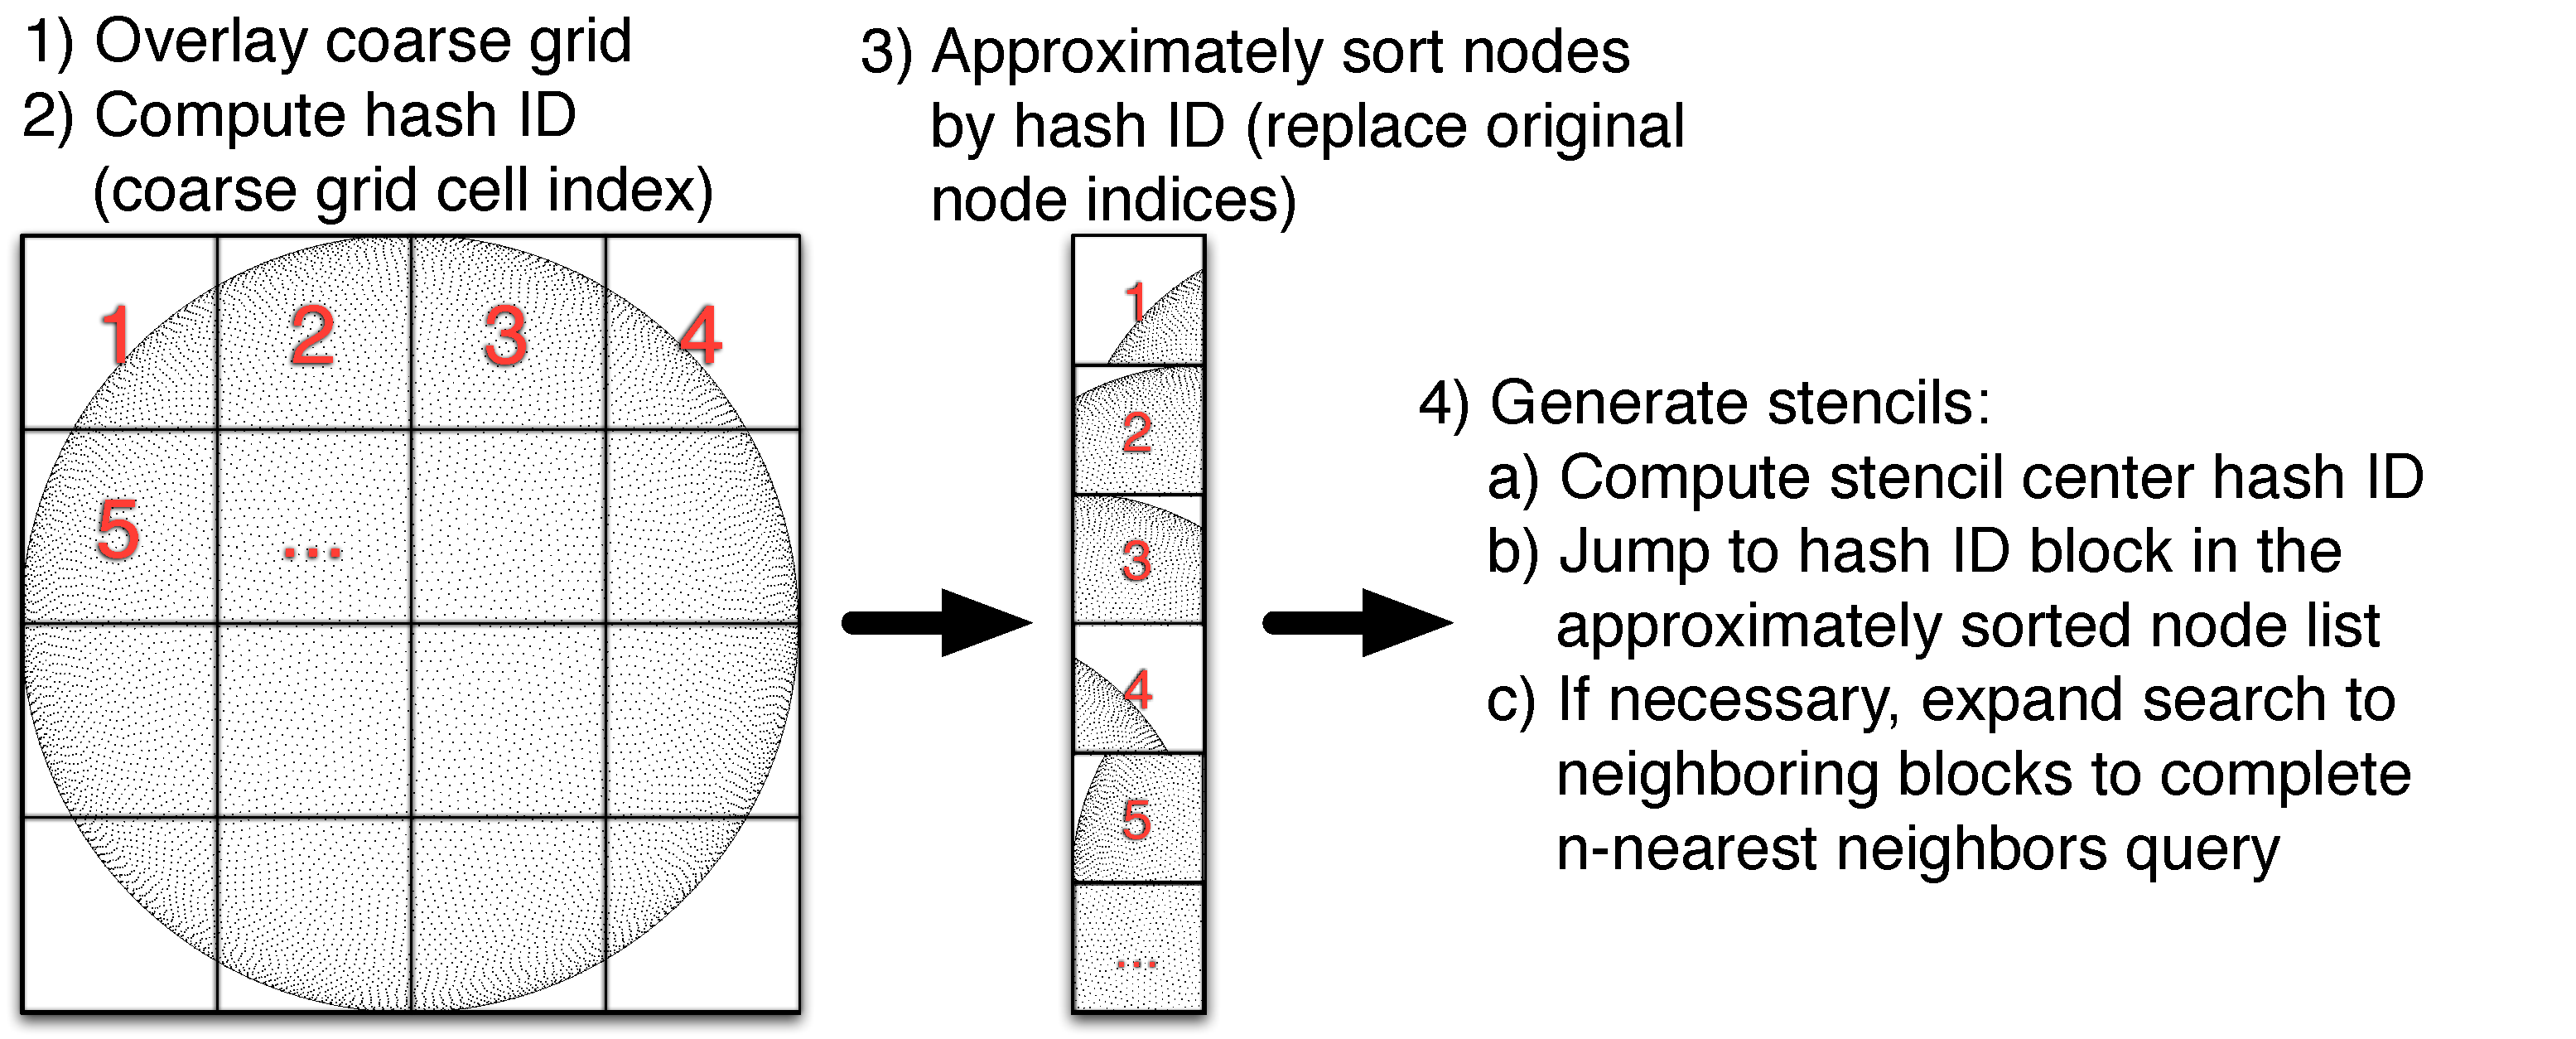
\includegraphics[width=1.0\textwidth]{../figures/chapter2/hashing_example/LSH_Concept.png}
\caption{High level overview of Locality Sensitive Hashing algorithm. First we overlay a coarse regular grid on the bounding box of the domain. The cells of the coarse grid cells are reordered in memory according to a space filling curve. Then we query neighbors by starting search with \authnote{Illustrate the query process} cell containing stencil center and append neighboring cells until stencil size $n$ nodes are found. We take $n$ closest neighbors (brute force search) if more than $n$ are appended to the list of candidates. }
\end{figure} 

\begin{figure}
\centering
\begin{subfigure}{0.425\textwidth}
\includegraphics[width=1.0\textwidth]{../figures/chapter2/hashing_example/bruteforce_N6400_n50-eps-converted-to.png}
\caption{k-D Tree} 
\end{subfigure} 
\begin{subfigure}{0.425\textwidth}
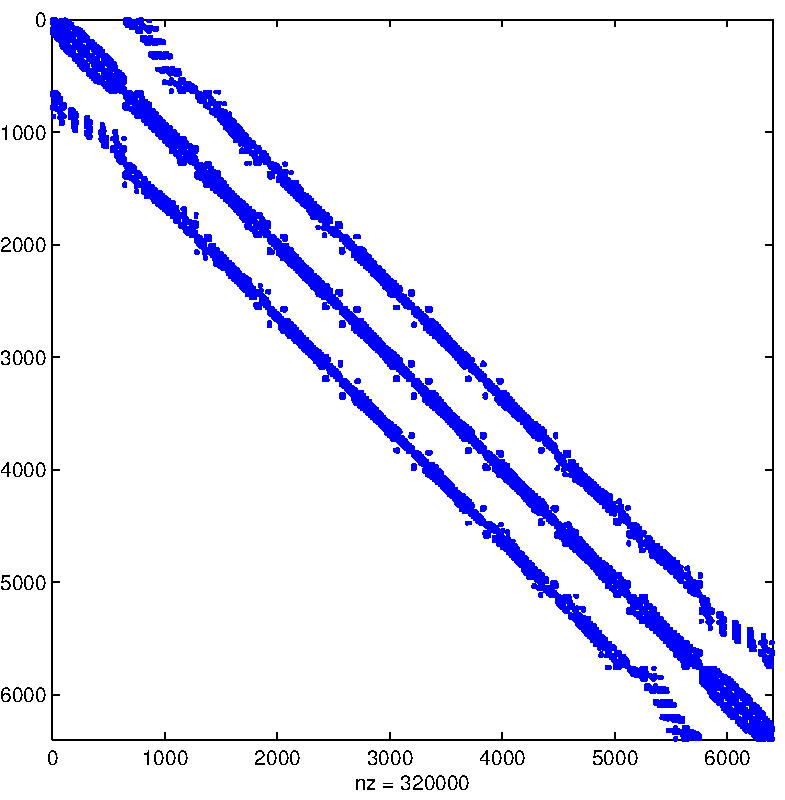
\includegraphics[width=1.0\textwidth]{../figures/chapter2/hashing_example/lsh_N6400_n50-eps-converted-to.png}
\caption{LSH}
\end{subfigure}
\caption{Example effects of node reordering within neighbor query algorithm for MD node set $N=6400$ with $n=50$. Matrix is $0.78\%$ full. k-D Tree maintains original ordering of the nodes and deceptively appears nearly dense. LSH algorithm reorders nodes according to raster ordering and reveals sparsity of the problem.  }
\end{figure} 

\section{Node Ordering}

Locality sensitive hashing also allows us to reorder the nodes

\cite{Saad2003} mentions the impact of ordering on conditioning.

Algorithms like Reverse Cuthill McKee and Approximate Minimum Degree ordering allow general restructuring of matrices. 

\authnote{NEed to compare conditioning of LSH and other algorithms in Matlab}

Q: what is an ideal ordering?
Q: what is the best conditioning from ordering?
Q: what is the relative cost of ordering?





\ifstandalone
\bibliographystyle{plain}
\bibliography{merged_references}
\end{document}
\else
\expandafter\endinput
\fi